\documentclass{assignment}
\ProjectInfos{光电子技术}{PHYS6651P}{2021-2022学年第一学期}{第九章作业}{}{陈稼霖}[https://github.com/Chen-Jialin]{SA21038052}

\begin{document}
\begin{prob}
    请说明光纤激光器的结构,它与光纤放大器的不同,以及光纤激光器和光纤放大器相比于传统器件有哪些有点.
\end{prob}
\begin{ans}
    
\end{ans}

\begin{prob}
    利用光纤中的非线性偏振演变效应,设计出一种被动锁模光纤激光器系统,其系统如下
    \begin{figure}[H]
        \centering
        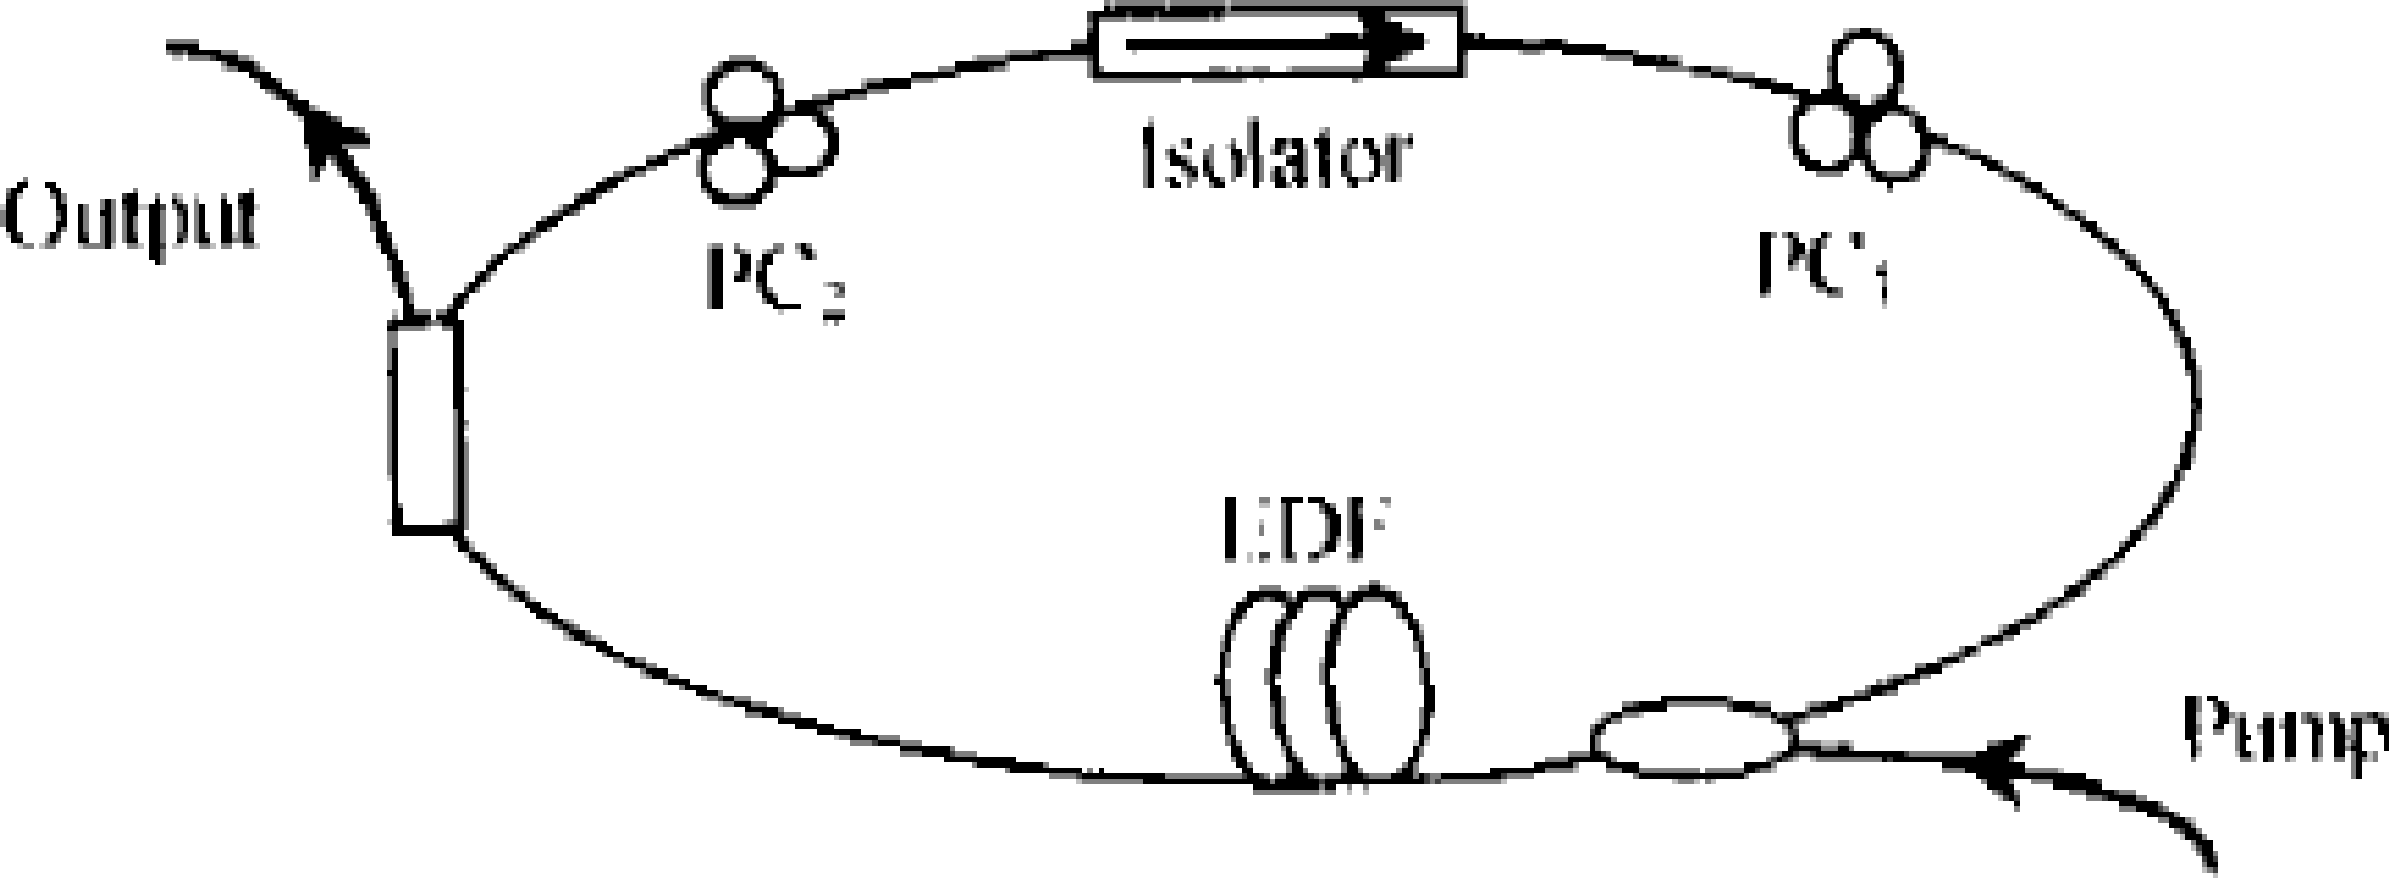
\includegraphics[width=.5\columnwidth]{5-1.png}
    \end{figure}
    PC1 和 PC2 是两块偏振控制器,试利用光纤中的偏振变化解释这种锁模光纤激光器的工作原理.
\end{prob}
\begin{ans}
    
\end{ans}
\end{document}